\section{Results}

\subsection{Historical Operation of \gls{EU} Reactors}


\begin{table}[h]
	\centering
	\scalebox{0.7}{
		\begin{tabular}{|c|c|c|c|}
			\hline
			Category & Unit & Value & Specifics\\ \hline
			Total UOX Usage & MTHM & 178,865 &  \\ \hline
			Total MOX Usage & MTHM & 8,909 & \\ \hline
			Total Used UOX Stored & MTHM & 157,472 & \gls{UNF} that are not reprocessed\\ \hline
			Total Used  MOX Stored & MTHM & 679 & \gls{UNF} that are not reprocessed \\ \hline
			Total Tailings & MTHM & 1,063,909 & \\ \hline
			Total Natural U Used & MTHM & 1,251,658 & \\ \hline
		\end{tabular}}
		\caption{Simulation Results for Historical Nuclear Operation of \gls{EU} Nations}
		\label{tab:sim_result}
		\end {table}
		
		\Cref{tab:sim_result} lists the important metrics
		obtained from the first simulation. The following
		values are the \gls{EU} inventory and history at year 2050.
		
		Figures \ref{fig:eu_num} and \ref{fig:eu_pow} display the
		timeseries of number of reactors and installed capacity in \gls{EU} nations.
		
		
		\begin{figure}[htbp!]
			\begin{center}
				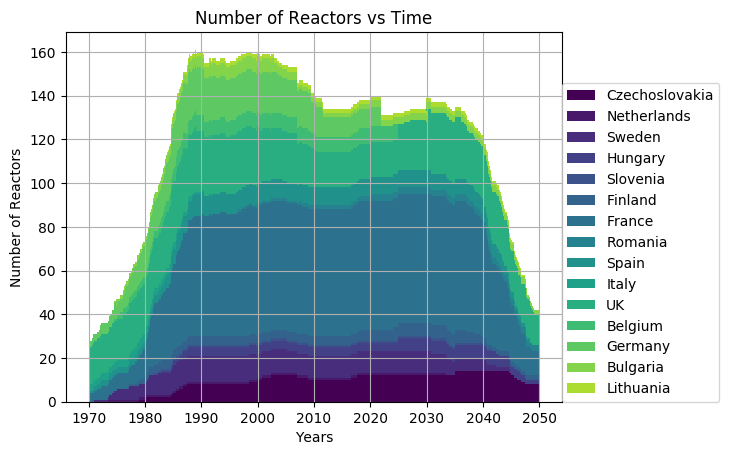
\includegraphics[width=\columnwidth]{./images/eu_future/number_plot.png}
			\end{center}
			\caption{Timeseries of number of reactors in \gls{EU}.}
			\label{fig:eu_num}
		\end{figure}
		
		\begin{figure}[htbp!]
			\begin{center}
				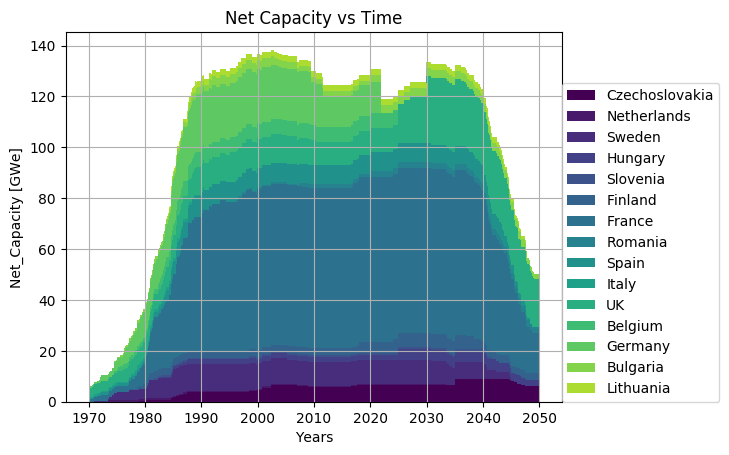
\includegraphics[width=\columnwidth]{./images/eu_future/power_plot.png}
			\end{center}
			\caption{Timeseries of installed nuclear capacity in \gls{EU}.}
			\label{fig:eu_pow}
		\end{figure}
		\FloatBarrier
		
		
		Figures \ref{fig:eu_tail} and \ref{fig:eu_snf} show the 
		timeseries of mass of tailings and used fuel accumulation in \gls{EU}.
		
		Figure \ref{fig:eu_fuel} shows the amount of fuel used in \gls{EU}.
		
		
		\begin{figure}[htbp!]
			\begin{center}
				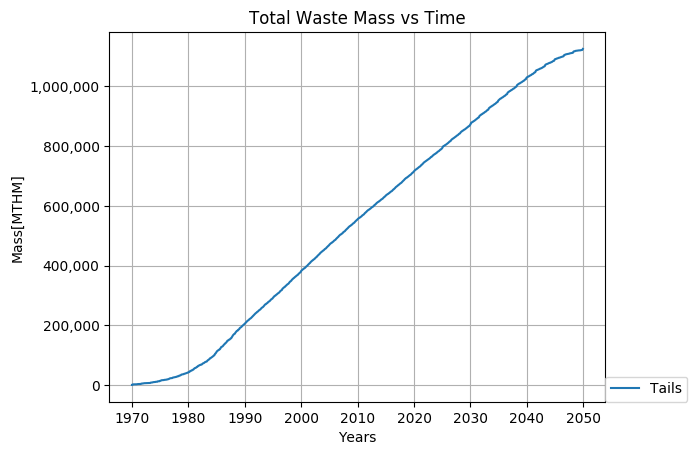
\includegraphics[width=\columnwidth]{./images/eu_future/tailings.png}
			\end{center}
			\caption{Timeseries of Tailings Mass in the \gls{EU}.}
			\label{fig:eu_tail}
		\end{figure}
		
		\begin{figure}[htbp!]
			\begin{center}
				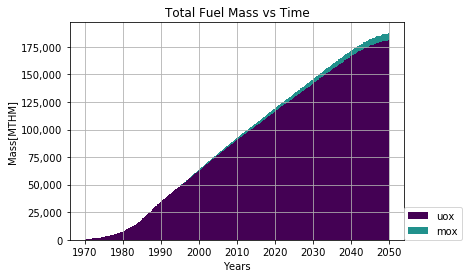
\includegraphics[width=\columnwidth]{./images/eu_future/total_fuel.png}
			\end{center}
			\caption{Timeseries of Total Fuel Usage in \gls{EU}.}
			\label{fig:eu_fuel}
		\end{figure}
		
		
		\begin{figure}[htbp!]
			\begin{center}
				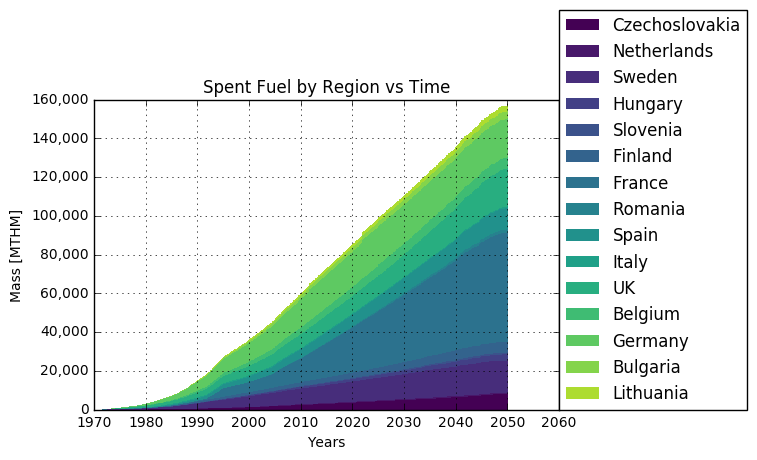
\includegraphics[width=\columnwidth]{./images/eu_future/snf.png}
			\end{center}
			\caption{Timeseries of Used Nuclear Fuel in \gls{EU}.}
			\label{fig:eu_snf}
		\end{figure}
		\FloatBarrier
		
		
		\begin{table}[h]
			\centering
			\begin{tabular}{|c|c|c|}
				\hline
				Isotope & Mass Fraction in Used Fuel [\%] & Quantity [t] \\ \hline
				Total & .9358 & 1,473 \\ \hline
				Pu238 & .0111 & 17.47 \\ \hline
				Pu239 & .518 & 815.7 \\ \hline
				Pu240 & .232 & 365.33 \\ \hline
				Pu241 & .126 & 198.41 \\ \hline
				Pu242 & .0487 & 76.68 \\ \hline
			\end{tabular}
			\caption{Plutonium From Used Fuel}
			\label{tab:pu}
		\end{table}
		
		
		To create \gls{MOX} for an ASTRID, 11\% Pu and 89\% depleted uranium is used.
		Thus $1,473$ tons of plutonium yields $13,390$ tons of
		\gls{MOX}. \Cref{tab:pu} lists the isotope, mass fraction,
		and quantity of plutonium that can be obtained from the 2050 \gls{UNF} inventory.
		
		
		\subsection{French \gls{SFR} Transition Scenario}
		
		From Varaine et al. \cite{marsaultmarie-sophie_pre-conceptual_2012}, a French
		ASTRID-type \gls{SFR} of capacity 600 MWe needs $1.225$ tons of
		plutonium a year, with an initial plutonium loading of $4.9$ tons. 
		Thus, the number of \glspl{SFR} that can be loaded with the reprocessed
		plutonium from \gls{UNF} can be estimated to $\frac{1,473}{4.9} \approx 300$ \glspl{SFR},
		assuming infinite reprocessing and fabrication capacity as well as
		abundant depleted uranium supply. 
		
		Also, assuming that \gls{MOX} can be recycled indefinitely,
		used \gls{MOX} from an ASTRID reactor
		contains enough plutonium to produce a \gls{MOX} fuel with
		the same mass, if mixed with depleted uranium. For example,
		used \gls{MOX} from an ASTRID reactor is assumed to be 12.6\% plutonium
		in this simulation (see \cref{tab:comp}), whereas a fresh \gls{MOX} is 11\% plutonium.
		Separating plutonium from used \gls{MOX} from
		an ASTRID reactor can create \gls{MOX} of the mass of used \gls{MOX}.
		The plutonium breeding ratio in this simulation is thus assumed to be
		$\approx 1.145$.
		
		The second scenario, with the tailings and used \gls{UOX}
		inventory, evaluates if the French can transition into \gls{SFR}
		without constructing additional \gls{LWR}s. This simulation
		assumed infinite reprocessing and fabrication capacity.
		
		\Cref{fig:fuel} shows the timeseries mass of \gls{MOX} used in the 
		\gls{SFR}s separated by their origin.
		Note that the plot shows \gls{MOX}
		accumulation prior to \gls{SFR} deployment from 2020.
		
		\begin{figure}[htbp!]
			\begin{center}
				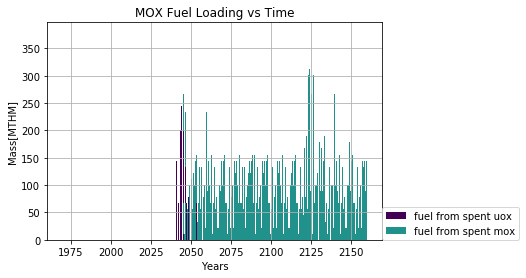
\includegraphics[width=\columnwidth]{./images/french-transition/where_fuel.png}
			\end{center}
			\caption{Timeseries of fuel used in the \gls{SFR}s [tons]}
			\label{fig:fuel}
		\end{figure}
		
		\Cref{fig:reprocess_waste} shows the amount of reprocessing waste
		(minor actinides, fission products) over time. Note that 
		reprocessing waste from \gls{UOX} reprocessing is substantially
		greater than waste from \gls{MOX} reprocessing due to its lower
		plutonium and uranium content.
		
		\Cref{fig:pu_isotopics} shows the isotopics of the plutonium that are
		reprocessed from the used fuel inventory.
		
		\begin{figure}[htbp!]
			\begin{center}
				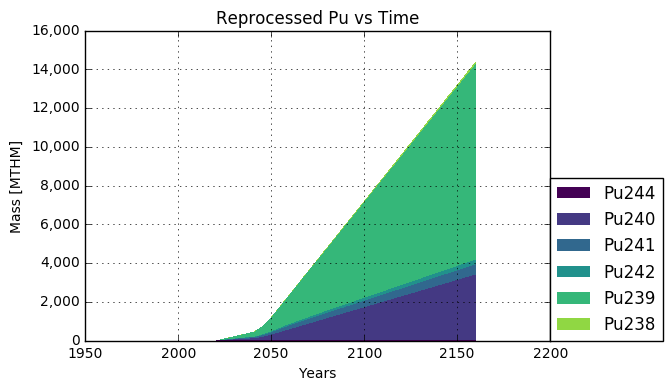
\includegraphics[width=\columnwidth]{./images/french-transition/rep_pu.png}
			\end{center}
			\caption{Plutonium timeseries separated by isotope}
			\label{fig:pu_isotopics}
		\end{figure}
		
		\begin{figure}[htbp!]
			\begin{center}
				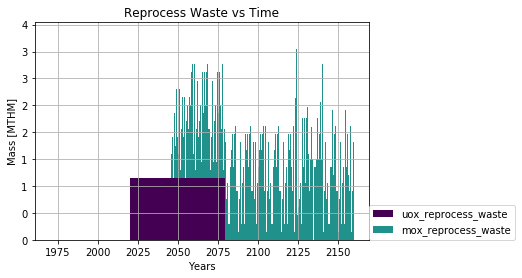
\includegraphics[width=\columnwidth]{./images/french-transition/reprocess_waste.png}
			\end{center}
			\caption{Reprocessing Waste for French Transition Scenario.}
			\label{fig:reprocess_waste}
		\end{figure}
		
		
		\begin{table}[h]
			\centering
			\scalebox{0.7}{
				\begin{tabular}{|c|c|c|}
					\hline
					Category & Unit & Value  \\ \hline
					Total MOX used & MTHM & 116,115  \\ \hline
					Total \glspl{SFR} Deployed & & 200 \\ \hline
					Total Plutonium Reprocessed & MTHM & 14,414 \\ \hline
					Total MOX from UOX Waste & MTHM & 9,729  \\ \hline
					Total MOX from MOX Waste & MTHM  & 150,426  \\ \hline
					Total Tailings used & MTHM & 105,664 \\ \hline
					Total legacy UNF reprocessed & MTHM & 97,298 \\ \hline
					Total Reprocessed Uranium Stockpile & MTHM & 251,100 \\ \hline
					Total Reprocess Waste & MTHM & 14,414 \\ \hline
				\end{tabular}}
				\caption {\gls{SFR} Simulation Results}
				\label{tab:sfr_sim_result}
				\end {table}
